%
% Foundations of Mathematics
%

\chapterimage{Philosophers.pdf}

\chapter{Foundations of Mathematics}
\label{chap:foundations_mathematics}

{\color{red} TODO: Introduce this chapter.}

Propositional logic deal with sentences, which can be true or false, and they way we can combine those sentences to construct arguments. Predicate logic extends propositional logic introducing quantified variables and relations, allowing richer arguments. Logic is studied here with the aim of providing the tools to examine the soundness, consistency and completeness of the axiomatic foundations of the theory of nescience. The exposition of logic contained in this chapter is a little bit unconventional. Most of the textbooks describing logic assume set theory, and the books on set theory require logic. We avoid this circularity by defining formulas as strings of symbols and logic as the rules to properly manipulate those strings. With this approach we loose the intuition behind logic, and the interpretability of the results. However, this book is about computers and automation, where meaning does not play a particular role.

{\color{red} TODO: Explain why if we have predicate logic to formalize the theory of nescience we also include type theory and category theory in this chapter.}

%
% Section: Propositional Logic
%

\section{Propositional Logic}

\emph{Propositional logic} is about the relationship between the truth of \emph{propositions}. Most of the authors require propositions to be declarative sentences, that is, they can be affirmed or denied. However, from a formal point of view, the content of propositions is not relevant to logic, and so, we will assume that any finite string of symbols can be a proposition. 

The language (syntax) of propositional logic contains two \emph{primitive symbols}, $\lnot$ and $\land$, called "\emph{not}" and "\emph{and}" respectively.  Propositions that do not contain those primitive symbols are called \emph{atomic sentences}. Atomic sentences are denoted by capital letters $A, B, C, \ldots$.

Formulas in propositional logic are derived from atomic sentences and primitive symbols.

\begin{definition}
\label{definition:logic_formula}
A finite string of symbols is a \emph{formula}, denoted by the capital letters $F, G, H, \ldots$, if and only if it is an atomic sentence or it is build up from atomic sentences by repeated application of the following two rules:
\begin{description}
\item[R1 (negation)] If $F$ is a formula, then $\lnot F$ is a formula.
\item[R2 (conjunction)] If $F$ and $G$ are formulas, then $( F \land G )$ is a formula.
\end{description}
\end{definition}

For example, the string $\lnot ( A \land (B \land C) )$ is a formula, but the string $ \lnot \land ( A \land B C ($ is not.

In order to make complex formulas easier to read (by humans), the following convenient abbreviations are introduced:

\begin{definition}
Let $F$ and $G$ be two formulas. The symbols $\lor$, $\rightarrow$ and $\leftrightarrow$, called "\emph{or}", "\emph{implies}" and "\emph{if and only if}" respectively, are defined as:
\begin{enumerate}[label=(\roman*)]
\item $\left( F \lor G \right)$ abbreviates $ \lnot \left( \lnot F \land \lnot G \right)$
\item $\left( F \rightarrow G \right)$ abbreviates $\left( G \lor \lnot F \right)$
\item $\left( F \leftrightarrow G \right)$ abbreviates $ \left( F \land \rightarrow G \right) \land \left( G \rightarrow F \right)$
\end{enumerate}
\end{definition}

Also, with readability in mind, the following notation is used:

\begin{notation}
If $F$ or $\left( F \right)$ is a formula, then the formulas $F$ and $\left( F \right)$ are considered as the same formula.
\end{notation}

If no parentheses are present, the symbol $\lnot$ has priority over the symbols $\land$, $\lor$, $\rightarrow$ and $\leftrightarrow$. For example, the formulas $\lnot ( A \land B )$ and $\lnot A \land B$ are different.

A subformula of a formula $F$ is a substring of $F$ that is itself a formula.

\begin{definition}
The \emph{subformulas} of a formula are defined as:
\begin{enumerate}[label=(\roman*)]
\item If $F$ is a formula, then $F$ is a subformula of itself. 
\item If $F$ is a formula and $G$ is a subformula of $F$, then $G$ is also a subformula of $\lnot F$. 
\item If $F$ and $G$ are formulas and $H$ is a subformula of $F$ or a subformula of $G$, then $H$ is also a subformula of $(F \land G)$.
\end{enumerate}
\end{definition}

From a semantic point of view, each formula has either a true value of \emph{true} or a true value of \emph{false}, represented by the symbols $1$ and $0$ respectively. The semantic of a formula is derived using \emph{true tables}. A true table is a table that given an assignment of values to atomic formulas allows us to derive the true value of more complex formulas.

The true table of the not symbol $\lnot$ is given by:

\begin{center}
\begin{tabular}{ c | c }
 $A$ & $\lnot A$ \\
 \hline
 $0$ & $1$  \\  
 $1$ & $0$    
\end{tabular}
\end{center}

The true table of the and symbol $\land$ is given by:

\begin{center}
\begin{tabular}{ c | c | c }
 $A$ & $B$ & $A \land B$ \\
 \hline
 $0$ & $0$ & $0$ \\
 $0$ & $1$ & $0$ \\
 $1$ & $0$ & $0$ \\
 $1$ & $1$ & $1$   
\end{tabular}
\end{center}

The true tables of more complex formulas can be derived by the repeated application of these two tables.

\begin{example}
The true table of the if-then, or implies, symbol $\rightarrow$ can be derived as follow:
\begin{center}
\begin{tabular}{ c | c | c | c }
 $A$ & $B$ & $\lnot A$ & $\lnot A \lor B$ \\
 \hline
 $0$ & $0$ & $1$ & $1$ \\
 $0$ & $1$ & $1$ & $1$ \\
 $1$ & $0$ & $0$ & $0$ \\
 $1$ & $1$ & $0$ & $1$
\end{tabular}
\end{center}
As we can observe in this table, a counterintuitive property of propositional logic is that a false statement implies anything.
\end{example}

Similar tables can be derived for the symbols $\lor$ and $\leftrightarrow$.

Let $A_1, \ldots, A_n$ be a list of $n$ atomic sentences, and let $\mathcal{F}(A_1, \ldots, A_n)$ denote all the formulas that can be built from those atomic sentences given Definition \ref{definition:logic_formula}. The list $A_1, \ldots, A_n$ is denoted by $\mathcal{S}$.

\begin{definition}
An \emph{assignment} of $\mathcal{S}$, denoted by $\mathcal{A}(\mathcal{S})$ or simply $\mathcal{A}$ if there is no doubt about the $S$ to which we are referring, is a mapping of the sentences of $\mathcal{S}$ to a list of $n$ true values. 
\end{definition}

An assignment $\mathcal{A}(\mathcal{S})$ can be extend to all the sentences of $\mathcal{F}(\mathcal{S})$ by means of computing the corresponding true tables. The true value of a sentence $F$ given the assignment $\mathcal{A}(\mathcal{S})$ is denoted by $\mathcal{A}(F)$.

\begin{definition}
If $\mathcal{A}(F)=1$ then it is said that $F$ \emph{holds} under assignment $\mathcal{A}$, or that $\mathcal{A}$ \emph{models} $F$, and it is denoted by $\mathcal{A} \models F$. A formula is \emph{satisfiable} if it holds under some assignment. A formula is \emph{valid}, denoted by $\models F$, if it holds under every assignment; a valid formula is called a \emph{tautology}. A formula is \emph{unsatisfiable} if it holds under no assignment; an unsatisfiable formula is called a \emph{contradiction}.
\end{definition}

\begin{example}
Next table shows that the formula $(A \lor B) \land (\lnot A \land \lnot B)$ is a contradiction.
\begin{center}
\begin{tabular}{ c | c | c | c | c | c | c}
 $A$ & $B$ & $A \lor B$ & $\lnot A$ & $\lnot B$ & $\lnot A \land \lnot B$ & $(A \lor B) \land (\lnot A \land \lnot B)$ \\
 \hline
 $0$ & $0$ & $0$ & $1$ & $1$ & $1$ & $0$ \\
 $0$ & $1$ & $1$ & $1$ & $0$ & $0$ & $0$ \\
 $1$ & $0$ & $1$ & $0$ & $1$ & $0$ & $0$ \\
 $1$ & $1$ & $1$ & $0$ & $0$ & $0$ & $0$
\end{tabular}
\end{center}
\end{example}

\begin{definition}
Let $F$ and $G$ be two formulas. It is said that $G$ is a \emph{consequence} of $F$, denoted by $F \models G$, if, and only if, $F \rightarrow G$ is a tautology, 
\end{definition}

It is easy to show that a formula $G$ is a consequence of formula $F$ if for every assignment $\mathcal{A}$, if $\mathcal{A} \models F$ then $\mathcal{A} \models G$.

\begin{definition}
Let $F$ and $G$ be two formulas. It is said that $F$ and $G$ are \emph{equivalent}, denoted by $F \equiv G$, if, and only if, $F \leftrightarrow G$ is a tautology.
\end{definition}

It is easy to show that if $G$ is a consequence of $F$ and $F$ is a consequence of $G$, then $F$ and $G$ are equivalent.

\begin{example}
The \emph{law of contraposition} states that $A$ implies $B$ is equivalent to not $B$ implies not $A$; with symbols $( A \rightarrow B ) \equiv ( \lnot B \rightarrow \lnot A )$. Next true table shows that $( A \rightarrow B ) \leftrightarrow ( \lnot B \rightarrow \lnot A )$ is a tautology.
\begin{center}
\begin{tabular}{ c | c | c | c | c | c | c}
 $A$ & $B$ & $A \rightarrow B$ & $\lnot B$ & $\lnot A$ & $\lnot B \rightarrow \lnot A$ & $(A \rightarrow B) \leftrightarrow (\lnot B \rightarrow \lnot A)$ \\
 \hline
 $0$ & $0$ & $1$ & $1$ & $1$ & $1$ & $1$ \\
 $0$ & $1$ & $1$ & $0$ & $1$ & $1$ & $1$ \\
 $1$ & $0$ & $0$ & $1$ & $0$ & $0$ & $1$ \\
 $1$ & $1$ & $1$ & $0$ & $0$ & $1$ & $1$
\end{tabular}
\end{center}
\end{example}

{\color{red}

Introduce and explain the following definition.

\begin{definition}
Let $\mathcal{F} = \{ F_1, F_2, ... \}$ be a set of formulas. For any assignment $\mathcal{A}$, we say $\mathcal{A}$ models $\mathcal{F}$, denoted by $\mathcal{A} \models \mathcal{F}$ if $\mathcal{A} \models F_i$ for each formula $F_i \in \mathcal{F}$. We say a formula $G$ is a consequence of $\mathcal{F}$, and write $\mathcal{F} \models G$, if $\mathcal{A} \models \mathcal{F}$ implies $\mathcal{A} \models G$ for every assignment $\mathcal{A}$
\end{definition}

}

{\color{red}

A proof system consists of a set of basic rules for derivations. These rules allow us to deduce formulas from sets of formulas. It may take several steps to derive a given formula $G$ from a set of formulas $\mathcal{F}$, where each step is an application of one of the basic rules. The list of steps forms a formal proof of $G$ from $\mathcal{F}$. 

We write $\mathcal{F} \vdash G$ to abbreviate "$G$ can be derived from $\mathcal{F}$.

A proof system is sound if the following property hold: if a formula $G$ can be derived from a set of formulas $\mathcal{F}$, then $G$ is a consequence of $\mathcal{F}$ (if $\mathcal{F} \vdash G$, then $\mathcal{F} \models G$).

If a proof system is sound, then it provides an alternative to truth tables for determining whether a formula $G$ is a consequence of a set of formulas $F$.

\begin{definition}
A formal proof in propositional logic is a finite sequence of statements of the form "$\mathcal{X} \vdash Y$" (where $\mathcal{X}$ is a set of formulas and $Y$ is a formula) each of which follows from the previous statemens by one of the rules in Table 1.5. We say that $G$ can be derived from $\mathcal{F}$ if there is a formal proof concluding with the statement $\mathcal{F} \vdash G$.
\end{definition}

}

{\color{red}

Formulas $F$ and $G$ are provably equivalent if both $\{ F \} \vdash G$ and $\{ G \} \vdash F$. If $F$ and $G$ are provably equivalent, then they are equivalent.

}

{\color{red} TODO: Proofs in the logic and proofs outside the logic.}

%
% Section: Predicate Logic
%

\section{Predicate Logic}
\label{sec:predicate_logic}

\emph{Predicate logic}, also known as \emph{first-order logic}, extends propositional logic with the use of variables and quantifiers over variables, in such a way that we can state the relation between non-logical objects. The language of predicate logic contains three \emph{primitive symbols}, the two symbols inherited from propositional logic $\lnot$, $\land$, and a new symbol $\exists$ called \emph{exists}. In this book we are interested in predicate logic with equality, and so, we add a fourth primitive symbol $=$ called \emph{equality}.

In propositional logic our object of study where formulas, that is, strings of symbols that follows well-defined syntactic rules. In predicate logic we also deal with formulas. The difference is that some of the symbols contained in formulas are distinguished because they play a special role. The distinguished symbols are :

\vskip 0.25cm

\begin{description}
\item [Variables] denoted by lower case letters from the end of the alphabet $(\ldots, x, y, z)$.
\item [Constants] denoted by lower case letters from the beginning of the alphabet $(a, b, c, \ldots)$. 
\item [N-ary functions] denoted by lower case letters $f, g$ and $h$.
\item [N-ary relations] denoted by upper case letters $P, Q, R$ and $S$.
\end{description}

\vskip 0.25cm

\begin{notation}
Given the limited number of letters of the alphabet, we can use subscripts to distinguish between the elements of formulas. For example, $x_1, x_2, x_3, \ldots$.
\end{notation}

The concept of N-ary function and and N-ary relation is better understood in the context of set theory. However, at this point we can not talk about sets, since the concept of set has not not been formally defined yet. As we will see in Section \ref{sec:set_theory}, in order to deal with sets, we have first to introduce a new symbol $\in$, and assume that some axioms (which are based on predicate logic) are true. By the moment, functions and relations are just distinguished symbols.

Next definition introduces the concept of \emph{term}, an intermediate step before to define the concept of \emph{formula}.

\begin{definition}
A finite string of symbols is a \emph{term} if and only if it is build up by repeated application of the following two rules:
\begin{description}
\item[T1] Every variable and every formula is a term.
\item[T2] If $f$ is an $N$-ary function and $t_1, t_2, \ldots, t_N$ are terms, then $f(t_1, t_2, \ldots, t_N)$ is also a term.
\end{description}
\end{definition}

Given the concept of term, we can formally define what we mean by atomic formula.

\begin{definition}
Let $t_1$ and $t_2$ be two terms, then the string $t_1 = t_2$ is an \emph{atomic formula}.
Let $R$ be a relation and $t_1, t_2, \ldots, t_N$ be $N$ terms, then the string $R(t_1, t_2, \ldots, t_N)$ is an \emph{atomic formula}.
\end{definition}

Formulas are built based on primitive symbols and atomic formulas. Recall rules \textbf{R1} and \textbf{R2} of Definition \ref{definition:logic_formula}. The same rules can be applied in predicate logic, together with a new rule. We use lower case Greek letters to denote formulas.

\begin{definition}
A string of symbols is a formula of first order logic if it is an atomic formula, or it can be derived by repeated application of the following rules:
\begin{description}
\item[R1] If $\varphi$ is a formula, then $\lnot \varphi$ is a formula.
\item[R2] If $\varphi$ and $\psi$ are formulas then $\varphi \land \psi$ is a formula.
\item[R2] If $\varphi$ is a formula and $x$ a variable then $\exists x \varphi$ is a formula.
\end{description}
\end{definition}

In predicate logic we also itroduce the following convenient abbreviation.

\begin{definition}
Let $x$ be a variable and $\varphi$ a formula. The symbol $\forall$, called \emph{for all}, is defined as:
\begin{enumerate}
\item $\forall x \varphi$ abbreviates $\lnot \exists x \lnot \varphi$.
\end{enumerate}
\end{definition}

\begin{example}
\end{example}

If no parenthesis are present, $\lnot$, $\exists$ and $\forall$ have priority over $\land$, $\lor$, $\rightarrow$ and $\leftrightarrow$.

In order to define the semantics of the symbols $\exists$ and $=$ we need the concept of \emph{structure}, since those symbols only make sense when they are associated with a structure. A structure consists of a underlying set together with an interpretation of the constants, functions and relations. However, in order to that, first we have to formally define what we mean by set.

%
% Set Theory
%
\section{Set Theory}
\label{sec:set_theory}

In this section we describe the ZFC axiomatic system for the theory of sets, named after the mathematicians Ernst Zermelo and Abraham Fraenkel. The 'C' in ZFC refers to the axiom of choice, also included in the initial list of axioms. ZFC is considered the standard form for axiomatic set theory, and it is the most common foundation of mathematics. An important point of ZFC is that all the entities in the universe of discource are sets, and so, elements that are not sets themselves are not allowed.

\begin{description}

\item[Axiom of Extensionality] If the set $x$ and the set $y$ have the same elements, then $x=y$.

\item[Axiom of Pairing] For any sets $a$ and $b$ there exist a set $\{a, b\}$ that contains exactly $a$ and $b$.

\item[Axiom Schema of Separation] If $P$ is a property with parameter $p$, then for any set $x$ and parameter $p$ there exists a set $y=\{u \in x : P(u,p) \}$ that contains all those sets $u \in x$ that have property $P$\footnote{It called axiom schema because there exists one axiom for each $P$.}.

\item[Axiom of Union] For any set $x$ there exists a set $y = \cup x$, the union of all elements of $x$. 

\item[Axiom of Power Set] For any set $x$ there exists a set $y = \mathcal{P}(x)$, the set of all subsets of $x$.

\item[Axiom of Infinity] There exists an infinite set.

\item[Axiom Schema of Replacement] If $F$ is a function, then for any set $x$ there exists a set $y = F(x) = \{F(u) : u \in x \}$. 

\item[Axiom of Regularity] Every nonempty set has an $\in$-minimal element.

\item[Axiom of Choice] Every family of nonempty sets has a choice function.

\end{description}


We denote by $\mathbb{N}$, $\mathbb{Z}$, $\mathbb{Q}$ and $\mathbb{R}$ the set of \emph{natural}\index{Set of natural numbers} numbers (including $0$), \emph{integers}\index{Set of integers}, \emph{rational}\index{Set of rationals} numbers and \emph{real}\index{Set of real numbers} numbers respectively. \emph{Positive integers}\index{Set of positive integers} are represented by $\mathbb{Z}^+$, and \emph{positive reals}\index{Set of positive reals} by $\mathbb{R}^+$ (in both cases the number $0$ is included). Let $A$ be a \emph{set}\index{Set}, by $x\in A$ we mean that $x$ is a \emph{member}\index{Member of a set} of $A$. The members of a set could be listed using brackets, for example $A = \{0, 1, 2, 3\}$, or the \emph{set formation}\index{Set formation notation} notation $A = \{x \in \mathbb{N} : x < 4\}$ (we require the \emph{universe}\index{Universe of a set} of the set to be known).

Let $A$ and $B$ be two sets, $A = B$ means that both sets are \emph{equal}\index{Equal sets}, $A \subset B$ that $A$ is a \emph{subset}\index{Subset} of $B$ but not equal, and $A \subseteq B$ that $A$ is a \emph{subset or equal} to $B$. Note that $A = B$ if, and only if, $A \subseteq B$ and $B \subseteq A$. The \emph{empty set}\index{Empty set} is denoted by $\varnothing$.

\begin{example}
For every set $A$ we have $\varnothing \subseteq A$ and $ A \subseteq A$.
\end{example}

The \emph{cardinality}\index{Cardinality of a set} of a finite set $A$, denoted by $d(A)$, is the number of elements of $A$. The cardinality of $\varnothing$ is 0. Given the sets $A$ and $B$, $A \cup B$ means the \emph{union}\index{Union of sets} of $A$ and $B$, and $A \cap B$ the \emph{intersection}\index{Intersection of sets} of $A$ and $B$. The union of $n$ sets $A_1, A_2, \ldots, A_n$ is represented by $\cup_{i=1}^n A_i$, and their intersection by $\cap_{i=1}^n A_i$. In case of an arbitrary collection of sets $I$ we use $\cup_{i \in I} A_i$ and $\cap_{i \in I} A_i$. And in case of an infinite collection of sets we use $\cup_{i}^{\infty} A_i$ and $\cap_{i}^{\infty} A_i$

Occasionally we will use \emph{Venn diagrams}\index{Venn diagram} to represent sets graphically (see Figure \ref{fig:Venn-diagram}).

\begin{figure}[h]
\centering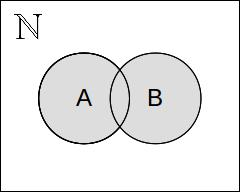
\includegraphics[scale=0.5]{Venn}
\caption{\label{fig:Venn-diagram}Representation of $A \cup B$ as a Venn Diagram}
\end{figure}

Given the sets $A$ and $B$, $A \backslash B$ is the \emph{set difference}\index{Set difference}, and ${A}^c$ is the \emph{complement}\index{Complement of a set} set of $A$. The \emph{De Morgan's laws} state that for every two sets $A$ and $B$ we have that $\left( A \cup B \right)^c = A^c \cap B^c$ and $\left( A \cap B \right)^c = A^c \cup B^c$.

Two sets $A$ and $B$ are \emph{disjoint}\index{Disjoint sets} if $A \cap B = \varnothing$. The sets $A_1, A_2, \ldots, A_n$ are disjoint if for every $i$ and $j$ such that $i \neq j$ we have that $A_i \cap A_j = \varnothing$. A \emph{partition}\index{Partition of a set} of a set $A$ is a collection of nonempty disjoint subsets of $A_1, A_2, \dots, A_n$ of $A$ such that  $A = \cup_{i=1}^n A_i$. The \emph{power set}\index{Power set} $\mathcal{P}(A)$ is the set whose members are all possible subsets of A. If $d(A)=n$ then $d\left( \mathcal{P}(A) \right) = 2^n$.

\begin{example}
Given the set $A = \{1, 2, 3\}$, its power set is:
\[
\mathcal{P}(A) = \{\varnothing, \{1\}, \{2\}, \{3\}, \{1,2\}, \{1,3\}, \{2,3\}, A\}
\]
\end{example}

% Relations

Given $x$ and $y$, the \emph{ordered pair}\index{Ordered pair} $\left(x, y\right)$ consists of $x$ and $y$ in that order. An \emph{n-tuple}\index{n-tuple} is an $n$-ary ordered pair. The \emph{Cartesian product}\index{Cartesian product} of two sets $A$ and $B$, denoted by $A \times B$, is the set composed by all the ordered pairs $\left(x, y\right)$ such that $x \in A$ and $y \in B$. The extension of the Cartesian product to $n$ sets $A_1, A_2, \dots, A_n$ is represented by $A_1 \times A_2 \times \dots A_n$, and the \emph{n-fold Cartesian product} of $A$ with itself is denoted by $A^n$.

A subset $R \subseteq A \times A$ is called a \emph{binary relation}\index{Binary relation}; we use the notation $aRb$ to denote that $\left(a, b\right) \in R$. A binary relation is called \emph{reflexive}\index{Reflexive relation} if for all $a \in A$ we have that $aRa$. A binary relation is called \emph{symmetric}\index{Symmetric relation} if for all $a, b \in A$ we have that if $aRb$ then $bRa$. A binary relation in which $aRb$ and $bRa$ implies that $a = b$ is called \emph{antisymmetric}\index{Antisymmetric relation}. A binary relation is \emph{transitive}\index{Transitive relation} if for all $a, b, c \in A$ we have that if $aRb$ and $bRc$ then $aRc$. A binary relation is called \emph{total}\index{Total relation} if for all $a, b \in A$ either $aRb$ or $bRa$. Binary relations can be extended to two different sets $A$ and $B$ as a subset $R \subseteq A \times B$, and to \emph{n-ary} relations $R \subseteq A_1 \times A_2 \times \dots A_n$.

A \emph{partial order} is a binary relation which is reflexive, transitive and antisymmetric; partial orders are represented by the symbol $\preceq$. A set with a partial order is called a \emph{partially ordered set} (also called a \emph{poset}). A relation that is is reflexive, transitive, antisymmetric and total is called a \emph{total order}; total orders are represented by the symbol $\leq$. A set paired with a total order is called a \emph{totally ordered set}\index{Totally ordered set}. Given a totally ordered set $A$ we denote $\max(A)$ the \emph{maximum}\index{Maximum} element of $A$, and $\min(A)$ its \emph{minimum}\index{Minimum} element.

\begin{example}
Let $R \subset \mathbb{N} \times \mathbb{N}$ a relation such that $(a, b) \in R$ if $a$ divides $b$. $\mathbb{N}$ with $R$ is a partially ordered set.
\end{example}

A \emph{function}\index{Function} is a binary relation $f \subseteq A \times B$ where for every $x \in A$ there is at most one $y \in B$ such that $\left(x, y\right) \in f$, the elements $\left(x, y\right) \in f$ are denoted by $f(x)=y$, and the function by $f : A \rightarrow B$. The set $A$ is called the \emph{domain}\index{Domain} of $f$, and $B$ the \emph{codomain}\index{Codomain}. The set $\{ y \in B : \exists x \in A , f(x) = y\}$ is the \emph{range}\index{Range} of $f$. A function is called \emph{partial}\index{Partial function} if the relation is not defined for all $x \in A$; we denoted by $f(x) \uparrow$ if the function $f$ is not defined for $x$. 

\begin{example}
The following C code defines a partial function from $\mathbb{R}$ to $\mathbb{R}$, since $inv(0)\uparrow$:
\begin{verbatim}
    double inv(double x) { return 1 / x }
\end{verbatim}
\end{example}

A function is \emph{injective}\index{Injective function} if for all $x$ and $y$ if $f(x) = f(y)$ then $x=y$. A function is \emph{surjective}\index{Surjective function} if for all $y$ there exists at least one $x$ such that $f(x) = y$. A function is \emph{bijective}\index{Bijective function} if it is both, injective and surjective. The \emph{identity}\index{Identity function} function $I_A : A \rightarrow A$, defined by $f(a) = a$ for all $a \in A$, is bijective. The concepts of function, partial function, injective, surjective and bijective can be easily generalized to $n$-ary relations.

Given a function $f$ the \emph{inverse}\index{Inverse function} function, denoted by $f^{-1}$, is defined by $f(f^{-1}(x)) = f^{-1}(f(x)) = x$. Given two functions $f$ and $g$, where the domain of $f$ is the range of $g$, we define the \emph{composition}\index{Composition} of $f$ with $g$, denoted by $f \circ g$, as $f \circ g = f(g(x))$.

An infinite set $A$ is \emph{countable}\index{Countable set} if there exists a bijective function between the elements of $A$ and the set of natural numbers $\mathbb{N}$. A set is \emph{uncountable}\index{Uncontable set} if it is neither finite nor countable. We say that a set has \emph{countable many}\index{Countable many set} elements if it is either finite or countable.

\begin{example}
$\mathbb{N}$, $\mathbb{Z}$ and $\mathbb{Q}$ are countable sets, $\mathbb{R}$ is not.
\end{example}

The \emph{characteristic function}\index{Characteristic function} of a set $A$ is the function $1_A : A \rightarrow \{1, 0\}$ defined as $1_A(x) = 1$ if $x \in A$ and $0$ otherwise.

Given a real number $x \in \mathbb{R}$, the \emph{absolute value}\index{Absolute value} of x, denoted $\mid x \mid$, is defined as $x$ is $x \geq 0$ and $-x$ if $x < 0$. The \emph{ceil}\index{Ceil} of $x$, denoted $\lceil x \rceil$ , is the least integer that is greater than or equal to $x$; the \emph{floor}\index{Floor} of $x$, denoted by $\lfloor x \rfloor$, is the greatest integer that is less than or equal to $x$. Given two positive integers $a$ and $b$, $a$ \emph{modulo} $b$, denoted by $a \bmod b$, is the remainder of the integer division of $a$ by $b$.

Let $f$ and $g$ be two functions $f,g:\mathbb{N}\rightarrow\mathbb{R}^{+}$. We say that $f(n)$ is of order of $g(n)$, denoted by $f(n)=O(g(n))$, if there exists positive integers $c$ and $m$ such that for every integer $n \geq m$ we have that $f(n)\leq cg(n)$. When $f(n)=O(g(n))$ we say that $g$ is an upper bound for $f$.


\section{Type Theory}

\section{Category Theory}


